\chapter{Spectral Geometry and Shape Analysis}
\label{ch:spectral_geometry}

%======================================================================
\section{Shape Spectra}
\label{sec:shape_spectra}

\subsection{Overview}
The spectrum of a shape\index{shape spectrum} refers to the set of eigenvalues of its Laplace--Beltrami operator\index{Laplace--Beltrami operator}. In geometric modeling, these eigenvalues (and their corresponding eigenfunctions\index{eigenfunction}) act as a ``geometric DNA'' or ``fingerprint'' that describes the intrinsic shape of a manifold. Shape space spectra are used for shape matching\index{shape matching}, classification, and analysis because they are invariant under isometric transformations\index{isometry invariance} (bending without stretching). The field is often summarized by the question posed by Mark Kac\index{Kac, Mark}: ``Can one hear the shape of a drum?''\index{can one hear the shape of a drum} \cite{kac1966}.

\subsection{Definitions}
\begin{definition}[Laplace--Beltrami Operator]\label{def:laplace_beltrami}
The Laplace--Beltrami operator\index{Laplace--Beltrami operator} $\Delta_M$ on a Riemannian manifold $(M, g)$ is the generalization of the Laplacian to curved spaces. In local coordinates, $\Delta_M f = \frac{1}{\sqrt{|g|}} \partial_i \left( \sqrt{|g|} \, g^{ij} \, \partial_j f \right)$, where $g_{ij}$ is the metric tensor and $|g|$ its determinant.
\end{definition}

\begin{definition}[Shape Spectrum]\label{def:shape_spectrum}
The shape spectrum is the non-decreasing sequence of eigenvalues $0 = \lambda_0 \le \lambda_1 \le \lambda_2 \le \cdots$ satisfying $\Delta_M \phi_k = \lambda_k \phi_k$ on a closed compact manifold $M$ of area $A$. The eigenvalues are also called the Dirichlet spectrum\index{Dirichlet spectrum}.
\end{definition}

\begin{definition}[Shape-DNA]\label{def:shape_dna}
Shape-DNA\index{Shape-DNA} is a shape descriptor formed by the first $k$ eigenvalues of the Laplace--Beltrami operator, typically normalized by the total area $\lambda_k \cdot A$ to enable comparison across differently-sized shapes \cite{reuter2006}.
\end{definition}

\begin{definition}[Heat Kernel]\label{def:heat_kernel}
The heat kernel\index{heat kernel} $K_t(x, y)$ on a manifold $M$ is the fundamental solution to the heat equation $\partial_t u = \Delta_M u$ with initial condition $u(0, x) = \delta(x)$. It admits the spectral expansion $K_t(x, y) = \sum_{k=0}^{\infty} e^{-\lambda_k t} \phi_k(x) \phi_k(y)$.
\end{definition}

\subsection{Theory}
The Laplacian spectrum encodes information about the area, perimeter, and topology of a shape.
\begin{enumerate}
  \item \textbf{Weyl's Law}\index{Weyl's law}: The growth rate of eigenvalues relates to the volume (area) of the shape: $\lambda_n \sim \frac{4\pi n}{Area}$ as $n \to \infty$ for a 2D domain.
  \item \textbf{Isometry Invariance}\index{isometry invariance}: Two isometric shapes have identical spectra. However, the converse is not always true (there exist non-isometric ``isospectral'' shapes\index{isospectral shapes} \cite{kac1966}).
  \item \textbf{Fundamental Tone}\index{Fiedler value}: $\lambda_1$ (the Fiedler value) relates to the ``width'' or ``length'' of the shape and is used for spectral clustering\index{spectral clustering} and graph partitioning\index{graph partitioning}.
\end{enumerate}

The spectrum is computed by discretizing the Laplacian on a mesh using \textbf{cotangent weights}\index{cotangent weights} and solving a generalized eigenvalue problem: $L \Phi = \Lambda M \Phi$, where $L$ is the stiffness matrix\index{stiffness matrix} and $M$ is the mass matrix\index{mass matrix}.

\begin{definition}[Cotangent Laplacian]\label{def:cotangent_laplacian}
The cotangent Laplacian\index{cotangent weights} discretizes $\Delta_M$ on a triangle mesh. For a vertex $i$ with one-ring neighbors $\{j\}$, the stiffness matrix entry is $L_{ij} = -\frac{1}{2}(\cot \alpha_{ij} + \cot \beta_{ij})$ for each edge $(i,j)$, where $\alpha_{ij}$ and $\beta_{ij}$ are the angles opposite to edge $(i,j)$ in the two adjacent triangles. The diagonal is $L_{ii} = -\sum_{j \ne i} L_{ij}$.
\end{definition}

\begin{theorem}[Weyl's Asymptotic Law]\label{thm:weyl_law}
For a bounded domain $\Omega \subset \mathbb{R}^2$ with area $|\Omega|$, the eigenvalues of the Dirichlet Laplacian satisfy
$$\lambda_n \sim \frac{4\pi n}{|\Omega|} \quad \text{as } n \to \infty.$$
\end{theorem}
\begin{proof}
The proof uses the phase-space counting argument (Weyl's original method\index{Weyl's law}). The number of eigenvalues $\le \lambda$ equals the number of lattice points $(k_1, k_2)$ satisfying $\frac{\pi^2 k_1^2}{L_1^2} + \frac{\pi^2 k_2^2}{L_2^2} \le \lambda$ for a rectangular domain. The area of this ellipse in $(k_1, k_2)$-space is $\frac{|\Omega|}{\pi^2} \cdot \pi \lambda = \frac{|\Omega| \lambda}{\pi}$, giving $N(\lambda) \sim \frac{|\Omega|}{4\pi} \lambda$. Inverting gives $\lambda_n \sim \frac{4\pi n}{|\Omega|}$. The result extends to arbitrary domains via a variational argument (comparing with inscribed/inscribed rectangles).
\end{proof}

\begin{remark}
Weyl's law\cref{thm:weyl_law} shows that the high-frequency part of the spectrum is determined entirely by the area, while lower eigenvalues encode finer geometric information (perimeter, topology, curvature). This motivates using only the first $k \ll N$ eigenvalues as shape descriptors.
\end{remark}

\begin{figure}[htbp]
\centering
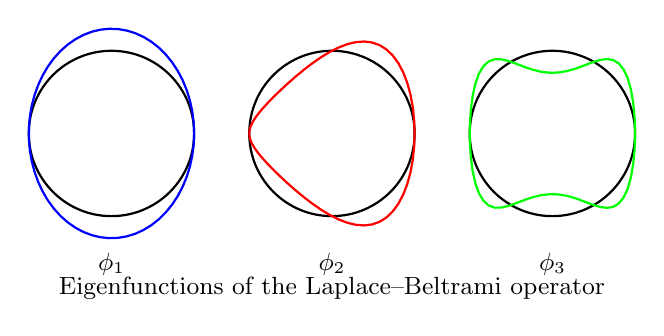
\begin{tikzpicture}[scale=0.7]
  % Eigenfunction phi_1
  \begin{scope}[xshift=0cm]
    \draw[thick] (0,0) circle (1.5);
    \draw[blue,thick,domain=0:360,samples=60] plot ({1.5*cos(\x)},{1.5*sin(\x)+0.4*sin(\x)});
    \node[below,font=\small] at (0,-2) {$\phi_1$};
  \end{scope}
  % Eigenfunction phi_2
  \begin{scope}[xshift=4cm]
    \draw[thick] (0,0) circle (1.5);
    \draw[red,thick,domain=0:360,samples=60] plot ({1.5*cos(\x)},{1.5*sin(\x)+0.4*sin(2*\x)});
    \node[below,font=\small] at (0,-2) {$\phi_2$};
  \end{scope}
  % Eigenfunction phi_3
  \begin{scope}[xshift=8cm]
    \draw[thick] (0,0) circle (1.5);
    \draw[green,thick,domain=0:360,samples=60] plot ({1.5*cos(\x)},{1.5*sin(\x)+0.4*sin(3*\x)});
    \node[below,font=\small] at (0,-2) {$\phi_3$};
  \end{scope}
  \node[font=\small] at (4,-2.8) {Eigenfunctions of the Laplace--Beltrami operator};
\end{tikzpicture}
\caption{First three eigenfunctions of the Laplacian on a circle. The eigenvalues $\lambda_k$ form the shape spectrum.}
\label{fig:shape_spectra}
\end{figure}


\subsection{Algorithm}
\begin{algorithm}
\caption{Shape-DNA Computation\index{Shape-DNA}\label{alg:shape_dna}}
\begin{algorithmic}[1]
\Function{ComputeShapeDNA}{$mesh, k$}
  \State $L, M \gets$ BuildDiscreteLaplacian($mesh$) \Comment{$L$: cotangent stiffness; $M$: lumped mass}
  \State $eigenvalues, eigenfunctions \gets$ \texttt{scipy.sparse.linalg.eigsh}($L, M, k{=}k, \sigma{=}{-}1e{-}6$)
  \State $area \gets mesh$.CalculateTotalArea()
  \State $normalized\_dna \gets eigenvalues \times area$
  \State \Return $normalized\_dna, eigenfunctions$
\EndFunction
\end{algorithmic}
\end{algorithm}

\begin{example}[Shape-DNA of a Unit Square]\label{example:shape_dna_square}
For a unit square $\Omega = [0,1]^2$ with Dirichlet boundary conditions\index{Dirichlet boundary condition}, the eigenvalues are $\lambda_{m,n} = \pi^2(m^2 + n^2)$ for $m, n \in \mathbb{Z}_{>0}$. The first five are:
\begin{itemize}
  \item $\lambda_{1,1} = 2\pi^2 \approx 19.74$ (fundamental tone)
  \item $\lambda_{1,2} = \lambda_{2,1} = 5\pi^2 \approx 49.35$ (doublet)
  \item $\lambda_{2,2} = 8\pi^2 \approx 78.96$
  \item $\lambda_{1,3} = \lambda_{3,1} = 10\pi^2 \approx 98.70$ (doublet)
\end{itemize}
The doublet structure reflects the four-fold symmetry\index{symmetry} of the square. For a rectangle of area 1 but side ratio $1:2$, the eigenvalues are $\pi^2(m^2 + 4n^2)$, and the first few differ, showing how the spectrum encodes aspect ratio.
\end{example}

\subsection{Parameter Selections}
\begin{itemize}
  \item \textbf{Number of Eigenvalues ($k$)}: Typically 10--100. More eigenvalues provide more detail but are more sensitive to mesh noise.
  \item \textbf{Normalization}\index{normalization}: Normalizing by $\lambda_1$ or the total area is necessary to compare shapes of different sizes\cref{def:shape_dna}.
  \item \textbf{Lumped vs.\ Consistent Mass}: Using a diagonal lumped mass matrix is faster and usually sufficient for shape analysis.
\end{itemize}

\subsection{Complexity}
\begin{itemize}
  \item \textbf{Matrix Construction}\index{matrix construction}: $O(F)$ where $F$ is the face count.
  \item \textbf{Eigen-decomposition}\index{eigen-decomposition}: $O(N^{1.5})$ for sparse matrices using Lanczos or LOBPCG methods.
  \item \textbf{Space Complexity}: $O(N \cdot k)$ to store the eigenfunctions.
\end{itemize}

\subsection{Usages}
\begin{itemize}
  \item \textbf{Shape Retrieval}\index{shape retrieval}: Searching a 3D database for models that ``look like'' a query object \cite{reuter2006}.
  \item \textbf{Symmetry Detection}\index{symmetry detection}: Identifying self-isometries of a shape.
  \item \textbf{Mesh Segmentation}\index{mesh segmentation}: Partitioning a mesh into functional parts based on the nodal sets of eigenfunctions.
  \item \textbf{Graph Partitioning}\index{graph partitioning}: Using the second eigenvector (Fiedler vector\index{Fiedler vector}) to split a mesh into two balanced pieces.
  \item \textbf{Style Analysis}: Classifying models into categories (e.g., ``human,'' ``animal,'' ``chair'') based on their spectral signatures \cite{levy2006}.
\end{itemize}

\subsection{Testing Methods and Edge Cases}
\begin{itemize}
  \item \textbf{Simple Geometries}: Verify that the spectrum of a sphere or a cube matches known analytical or high-precision values\cref{example:shape_dna_square}.
  \item \textbf{Area Invariance}: Ensure that scaling a mesh and then normalizing the spectrum yields the same DNA\cref{def:shape_dna}.
  \item \textbf{Mesh Refinement}: Verify that the eigenvalues converge as the mesh resolution increases.
  \item \textbf{Disconnected Components}: The number of zero eigenvalues ($\lambda=0$) should match the number of connected components\index{connected component}.
  \item \textbf{Isospectral Shapes}\index{isospectral shapes}: Test on known pairs of isospectral shapes (like the ``drums'' of Gordon, Webb, and Wolpert\cite{kac1966}) to see if they can be distinguished by other means.
\end{itemize}

\subsection{References}
\begin{itemize}
  \item Kac, M. (1966). ``Can one hear the shape of a drum?'' \textit{American Mathematical Monthly} \cite{kac1966}.
  \item Reuter, M., Wolter, F.\,E., \& Peinecke, N. (2006). ``Laplace--Beltrami spectra as `Shape-DNA' of surfaces and solids.'' \textit{Computer-Aided Design} \cite{reuter2006}.
  \item Levy, B. (2006). ``Laplace-Beltrami Eigenfunctions towards an Optimal Tool for Geology and Geometry.'' \textit{SMA} \cite{levy2006}.
  \item Botsch, M., et al. (2010). ``Polygon Mesh Processing.'' AK Peters \cite{botsch2010}.
  \item Wikipedia: Spectral shape analysis.
\end{itemize}

%======================================================================
\section{Shape Space Spectra}
\label{sec:shape_space_spectra}

\subsection{Overview}
Shape Space Spectra (or SpectralNet\index{SpectralNet}) is a deep-learning-based framework for learning spectral descriptors for shape analysis \cite{sharp2025}.

Traditional spectral descriptors (like HKS\index{Heat Kernel Signature} or WKS\index{Wave Kernel Signature}) are based on the Laplace--Beltrami spectrum of a single shape. Shape Space Spectra learns how these descriptors change as a shape is deformed. This provides a more robust way to perform tasks like shape matching and retrieval across non-rigid shapes \cite{bronstein2017}.

\begin{definition}[Shape Space Descriptor]\label{def:shape_space_descriptor}
A shape space descriptor is a learned map $f_\theta: (x, \theta) \mapsto \mathbb{R}^k$ that takes a point $x$ on a surface and a deformation parameter $\theta$, and produces a $k$-dimensional spectral descriptor. The parameters $\theta$ are learned end-to-end to maximize discriminability across non-rigid shape correspondences.
\end{definition}

\subsection{Implementation Details}
In \texttt{CompGeom}, the \texttt{ShapeSpaceSpectralNet} provides:
\begin{enumerate}
  \item \textbf{Point-Cloud Basis}\index{point cloud}: Operates on 3D point cloud representations of shapes.
  \item \textbf{Latent Deformations}: Integrates shape deformation parameters ($\theta$) to learn how the spectrum responds to change.
  \item \textbf{Eigen-Descriptor Computation}: Generates $k$ spectral descriptors for each point.
\end{enumerate}

\begin{remark}
The key advantage of shape space spectra over fixed descriptors (like Shape-DNA\cref{def:shape_dna}) is that the learned descriptors adapt to the distribution of deformations encountered in a dataset, rather than relying on a fixed spectral truncation. This makes them more robust to noise, partial observations, and topology changes.
\end{remark}

\subsection{Usage}
\begin{algorithm}
\caption{Shape Space SpectralNet Usage\index{SpectralNet}\label{alg:shape_space_spectralnet}}
\begin{algorithmic}[1]
\State \texttt{from compgeom.mesh.algorithms.shape\_space\_spectra import ShapeSpaceSpectralNet}
\State \texttt{import torch}
\Statex
\State \texttt{\# num\_eigen: number of spectral descriptors to learn}
\State \texttt{net = ShapeSpaceSpectralNet(num\_eigen=10)}
\Statex
\State \texttt{\# x: point cloud (N, 3), theta: deformation parameters (N, D)}
\State \texttt{x = torch.randn(100, 3)}
\State \texttt{theta = torch.randn(100, 8)}
\State \texttt{descriptors = net(x, theta)}
\end{algorithmic}
\end{algorithm}

\begin{example}[Shape Space Spectra on a Bent Cylinder]\label{example:shape_space_cylinder}
Consider a cylinder that is gradually bent from straight to U-shaped, parameterized by a bending angle $\theta \in [0, \pi]$. Traditional Shape-DNA\cref{def:shape_dna} changes as the cylinder bends (because the spectrum shifts), but the changes are global and non-local. A shape space spectral descriptor $f_\theta(x, \theta)$ learns to produce stable per-vertex features: at $\theta = 0$ (straight cylinder), the descriptor is uniform along the axis; as $\theta$ increases, the descriptor for points on the inner bend diverges from those on the outer bend, capturing the local geometric distortion in a way that is invariant to isometric deformation.
\end{example}

\subsection{References}
\begin{itemize}
  \item Sharp, N., et al. ``SpectralNet: Learning Spectral Descriptors for Shape Analysis.'' \textit{ACM Transactions on Graphics (SIGGRAPH)}, 2025/2026 \cite{sharp2025}.
  \item Bronstein, M.\,M., et al. ``Geometric Deep Learning: Grids, Groups, Graphs, Geodesics, and Gauges.'' 2017 \cite{bronstein2017}.
\end{itemize}

%======================================================================
\section{Odeco Frame Fields}
\label{sec:odeco_frame_fields}

\subsection{Overview}
Odeco Frame Fields\index{Odeco frame fields} is a method for designing 3D anisotropic frame fields\index{frame field} in tetrahedral meshes\index{tetrahedral mesh} using Orthonormal Decomposable (Odeco) tensors\index{Odeco tensor} \cite{zhu2025}.

A frame field is a volumetric structure that assigns a 3D orthogonal frame to each point in a volume. Frame fields are essential for generating high-quality quad-dominant or hex-dominant meshes\index{hex meshing}\index{quad meshing}. Standard frame field representations (like 4th-order tensors) can be difficult to control. The Odeco representation provides a more direct way to specify the orientation and stretching of the local frame \cite{panozzo2014}.

\begin{definition}[Odeco Tensor]\label{def:odeco_tensor}
An Orthonormal Decomposable (Odeco) tensor $\mathbf{Q} \in \mathbb{R}^{3 \times 3}$ is a symmetric positive-definite tensor that admits an eigendecomposition $\mathbf{Q} = \mathbf{R} \, \text{diag}(\sigma_1, \sigma_2, \sigma_3) \, \mathbf{R}^T$, where $\mathbf{R} \in SO(3)$ is a rotation matrix and $\sigma_1 \ge \sigma_2 \ge \sigma_3 > 0$ are the principal stretching factors. The eigenvectors of $\mathbf{Q}$ define the local frame.
\end{definition}

\begin{definition}[Frame Field]\label{def:frame_field}
A frame field on a tetrahedral mesh $\mathcal{T}$ is a map $\mathcal{F}: \mathcal{T} \to SO(3) \times \mathbb{R}_{>0}^3$ assigning to each tetrahedron a rotation (orientation) and three stretching magnitudes (anisotropy\index{anisotropy}). Equivalently, it can be represented as an Odeco tensor field $\{\mathbf{Q}_e\}$ over the edges or elements of $\mathcal{T}$.
\end{definition}

\subsection{Implementation Details}
The \texttt{OdecoFrameField} implementation in \texttt{CompGeom} allows for:
\begin{enumerate}
  \item \textbf{Boundary Alignment}\index{boundary alignment}: The frames can be explicitly aligned to boundary normals.
  \item \textbf{Anisotropy Control}: The stretching magnitudes along each frame axis can be specified.
  \item \textbf{Smoothness Optimization}\index{smoothness optimization}: The orientations and stretching can be propagated through the volume via a smoothing process.
\end{enumerate}

\begin{theorem}[Odeco Frame Field Smoothness]\label{thm:odeco_smoothness}
The Odeco frame field smoothness energy $E_{\text{smooth}} = \sum_{(e_1, e_2) \in \mathcal{E}} w_{e_1,e_2} \|\mathbf{Q}_{e_1} - \mathbf{R}_{e_1 \to e_2} \, \mathbf{Q}_{e_2} \, \mathbf{R}_{e_1 \to e_2}^T\|^2$ is minimized when adjacent frames are related by parallel transport\index{parallel transport} along the mesh, where $\mathbf{R}_{e_1 \to e_2}$ is the rotation that maps the reference frame of $e_1$ to that of $e_2$.
\end{theorem}
\begin{proof}
The energy measures the Frobenius norm of the difference between the tensor at $e_1$ and the parallel-transported tensor from $e_2$. Since the Frobenius norm is invariant under simultaneous rotation $\|\mathbf{A}\|_F = \|\mathbf{R}\mathbf{A}\mathbf{R}^T\|_F$, the energy is well-defined regardless of the choice of reference frame for each element. The global minimizer of this quadratic energy is the solution to a sparse linear system on the mesh, which can be solved efficiently by preconditioned conjugate gradient\index{conjugate gradient}.
\end{proof}

\subsection{Usage}
\begin{algorithm}
\caption{Odeco Frame Field Design\index{Odeco frame fields}\label{alg:odeco_frame_field}}
\begin{algorithmic}[1]
\State \texttt{from compgeom.mesh.volume.odeco\_frame\_field import OdecoFrameField}
\State \texttt{from compgeom.mesh.volume.tetmesh.tetmesh import TetMesh}
\State \texttt{import numpy as np}
\Statex
\State \texttt{\# Load a tetrahedral mesh}
\State \texttt{mesh = TetMesh.from\_file("volume.obj")}
\Statex
\State \texttt{\# Initialize and align to boundary}
\State \texttt{off = OdecoFrameField(mesh)}
\State \texttt{off.align\_to\_boundary(normals, indices)}
\Statex
\State \texttt{\# Propagate across the volume}
\State \texttt{off.solve\_smoothness(iterations=10)}
\end{algorithmic}
\end{algorithm}

\begin{example}[Frame Field on a Cube]\label{example:odeco_cube}
Consider a unit cube meshed with tetrahedra. We align the boundary faces to the coordinate axes: the front/back faces have frame $(e_1, e_2, e_3) = (x, y, z)$, the left/right faces have $(y, z, x)$, and the top/bottom have $(z, x, y)$. The Odeco smoothness solver\cref{thm:odeco_smoothness} propagates these orientations into the interior, creating a smoothly varying frame field. The resulting field has a singularity\index{frame field singularity} at the cube center (since the four boundary orientations cannot be globally consistent), which is detected as a point where the frame rotation is ill-defined. This singularity structure guides the subsequent hexahedral remeshing\index{hexahedral remeshing}.
\end{example}

\begin{remark}
Frame field singularities\index{frame field singularity} are analogous to vector field singularities on surfaces (Poincar\'{e}--Hopf theorem\index{Poincar\'{e}--Hopf theorem}). Their number and type are constrained by the Euler characteristic\index{Euler characteristic} of the domain. Controlling singularity placement is critical for generating high-quality hex meshes \cite{bommes2013}.
\end{remark}

\subsection{References}
\begin{itemize}
  \item Zhu, Y., et al. ``Designing 3D Anisotropic Frame Fields with Odeco Tensors.'' \textit{ACM Transactions on Graphics (SIGGRAPH)}, 2025 \cite{zhu2025}.
  \item Panozzo, D., et al. ``Frame Fields: An Orientation-aware Surface Representation.'' \textit{ACM Transactions on Graphics (SIGGRAPH)}, 2014 \cite{panozzo2014}.
  \item Bommes, D., et al. (2013). ``Quad-Mesh Generation and Processing: A Survey.'' \textit{Computer Graphics Forum} \cite{bommes2013}.
\end{itemize}
